\section{Introduction}

\begin{frame}{Beyond expected values}

	Many settings require that a \alert{risk profile} is imposed:
	\begin{itemize}
		\item Expected values assume a \alert{risk neutral} stance;
		\item Risk neutral means that the product \alert{probability $\times$ outcome} is the single factor under consideration.	
	\end{itemize}
	
	\pause
	In many settings, the decision-maker may have other implicit priorities:
		\begin{itemize}
			\item Impose (probabilistic) guarantees on \alert{feasibility} \\ $ \Rightarrow$ {\bf chance constraints};
			\item Avoid being exposed to the possibility of a \alert{high-loss} \\ $\Rightarrow$ {\bf risk measures}.	
		\end{itemize}
 
\end{frame}


\section{Chance constraints}


\begin{frame}{Feasibility guarantees}

	A solution may \alert{reveal itself infeasible} once the uncertainty unveils
	\vspace{-6pt}
	\begin{itemize}
		\item Particularly critical in settings where \alert{infeasibility} has a high penalty;
		\item Appealing in settings in which \alert{safety and resilience} are requirements.	
	\end{itemize}
	
	\pause
	Let us first consider the case \alert{without} recourse. Our problem is thus
	%
	\begin{align*}
		\mini & c^\top x  \\
		\st  & Ax = b \\
			 & T(\xi)x	= h(\xi), \ \forall \xi \in \Xi \\
		     & x \ge 0. 
	\end{align*}
	%
	\pause
	Notice the \alert{static} nature of the problem 
	\vspace{-6pt}
	\begin{itemize}
		\item once a decision $x$ is made, we observe the realisation of the uncertainty $\xi$;
		\item no correction decision is allowed.
	\end{itemize} 
	
\end{frame}


\begin{frame}{Feasibility guarantees}
	
	There are two main paradigms on how to model feasibility requirements for the constraint $T(\xi)x	= h(\xi), \ \forall \xi \in \Xi$:
	\begin{enumerate}
		\item Impose that $T(\xi)x	= h(\xi)$ holds for \alert{a set of realisations} $U \subseteq \Xi$ (robust optimisation)
		\item Impose that the \alert{probability} of $T(\xi)x	= h(\xi)$ holding is at least a given threshold (chance constraints)
	\end{enumerate}
	%
	As one may suspect, the two approaches are \alert{interrelated}. 
	
	\pause
	Imposing a chance constraint means that a solution is deemed \alert{acceptable} if, for a given confidence level $\alpha$, we have that
	%
	\begin{equation*}
		\mathbb{P}(T(\xi)x = h(\xi)) \ge \alpha.
	\end{equation*} 
		
\end{frame}


\begin{frame}{Types of chance constraints}

	Let $T(\xi)$ be a $m_2 \times n_1$ matrix, where $T(\xi)_i$ represents its $i^{\text{th}}$-row, and $h(\xi)$ a $m_2$ vector with components $h(\xi)_i$. 

	There are two types of chance constraints:
	\begin{enumerate}[<+->]
		\item {\bf Individual chance constraints} (ICC):
		\begin{equation*}
			p_i(x) := \mathbb{P}((T(\xi)_i)^\top x = h(\xi)_i) \ge \alpha_i, \ \forall i \in [m_2],
		\end{equation*}
		\item {\bf Joint chance constraints} (JCC):
		\begin{equation*}
			p(x) := \mathbb{P}((T(\xi)_i)^\top x = h(\xi)_i, \ \forall i \in [m_2]) \ge \alpha
		\end{equation*}
	\end{enumerate}
	%
	\vspace{-15pt}
	{\onslide<+->
	JCCs are typically more challenging from a tractability standpoint
	\vspace{-6pt}
	\begin{itemize}
		\item ICCs can be used to \alert{approximate} a JCC;
		\item {\bf Bonferroni inequality}: for a given $x$, if $p_i(x) > \alpha_i$, $\forall i \in [m_2]$, where $\alpha_i = 1 - \frac{(1-\alpha)}{m_2}$, then $p(x) \ge \alpha$.   		
	\end{itemize}
	}
\end{frame}


\begin{frame}{Tractability of chance constraints}
	
	Tractability issues stem from the properties of the \alert{feasible sets} generated by chance constraints. Let
	\begin{align*}
		& C(\alpha_1, \dots, \alpha_{m_2}) := \bigcap_{i \in [m_2]} = C_i(\alpha_i), \text{ where } \\
		& C_i(\alpha_i) = \braces{x \in \reals^n : p_i(x) \ge \alpha_i}.
	\end{align*}
	%
	\vspace{-18pt}
	\begin{itemize}
		\item No general result that guarantees the \alert{convexity} of $C_i(\alpha_i)$;
		\item \alert{Particular cases} do exist for important distributions which lead to the convexity of $C(\alpha_1, \dots, \alpha_{m_2})$.
	\end{itemize} 
	
	\pause
	For example, assume that $T(\xi) = T$, $\forall \xi \in \Xi$, and that $h(\xi) = \xi$. For the univariate case, we have that
		\begin{equation*}
			C(\alpha) = \braces{x \in \reals^{n_1} :  Tx \ge F^{-1}(\alpha)}.
		\end{equation*}
\end{frame}



\begin{frame}{Tractability of chance constraints}

	One general result that is known and can be informative in the multivariate case is the following:
	%
	\begin{theorem}
		Let $T(\xi) = T$, $\forall \xi \in \Xi$, and $h(\xi) = \xi$, where $\xi \in \reals^{m_2}$ is a random vector with density function $f$. If $\log(f)$ is concave (assuming $\log(0) = -\infty$), then $C(\alpha)$ is closed and convex for all $\alpha \in [0,1]$.
	\end{theorem}
	\pause
	\begin{itemize}
		\item {\bf Main case:} $\xi \sim \text{Normal}(\mu, \Sigma)$ with vector mean $\mu$ and covariance matrix $\Sigma$;
		\item Uniform case also ``trivial'' to show that holds;	
		\item For a list of ``other distributions'': \cite{nemirovski2007convex}
	\end{itemize}

	
\end{frame}



\begin{frame}{Tractability of chance constraints}

	Another important known case is this: $T(\xi)$ is a $1 \times n$ random vector and $h(\xi) = h$, $\forall \xi \in \Xi$.
	
	\begin{theorem}
		Assume that $T(\xi) = \xi = (\xi_i)_i=1^{n_1}$ is the only random parameter, where $\xi \sim \text{Normal}(\mu, \Sigma)$ with $\mu = (\mu_i)_{i=1}^{n_1}$ a vector of means and $\Sigma$ 	the covariance matrix. Then
		\begin{equation*}
			C(\alpha) = \braces{x \in \reals^{n_1} : \mu^\top x \ge h + \Phi^{-1}(\alpha)\sqrt{x^\top \Sigma x}}
		\end{equation*}
	\end{theorem}
	
\end{frame}


\begin{frame}{Tractability of chance constraints}

	\begin{proof} 
		The random variable $\xi^\top x$ is a multivariate normal with mean $\mu^\top x$ and variance $x^\top\Sigma x$. Letting $Z$ follow a standard normal, we have that
		\vspace{-6pt}
		{\small
		\begin{align*} 
		 \mathbb{P}(\xi^\top x \ge h) \ge \alpha & \Leftrightarrow \mathbb{P}\left(\frac{\xi^\top x - \mu ^\top x}{\sqrt{x^\top \Sigma x}} \ge \frac{h^\top x - \mu ^\top x}{\sqrt{x^\top \Sigma x}} \right) \ge \alpha \\
		 & \Leftrightarrow 1 - \mathbb{P}\left( Z \le \frac{h - \mu ^\top x}{\sqrt{x^\top \Sigma x}} \right) \ge \alpha	\\
		 & \Leftrightarrow 1 - \Phi\left(\frac{h - \mu ^\top x}{\sqrt{x^\top \Sigma x}} \right)	\ge \alpha \\
		 & \Leftrightarrow \Phi\left(\frac{\mu ^\top x - h}{\sqrt{x^\top \Sigma x}} \right)	\ge \alpha\\
		 & \Leftrightarrow \frac{\mu ^\top x - h}{\sqrt{x^\top \Sigma x}} \ge \Phi^{-1}(\alpha) \Leftrightarrow \mu^\top x \ge h + \Phi^{-1}(\alpha)\sqrt{x^\top \Sigma x} \qedhere
		\end{align*}}
		Notice that the constraint is convex if $\Phi^{-1}(\alpha) \ge 0$, i.e., $\alpha \in [1/2, 1]$.
	\end{proof}
	
\end{frame}


\begin{frame}{Discretisation of chance constraints}

	An alternative way of handling chance constraints is using \alert{scenarios}:
	\begin{itemize}
		\item Allows for general (discrete) distributions;	
		\item \alert{Convex} problems by construction (for an originally convex problem);
		\item Allows for recourse decisions;
		\item Requires \alert{binary variables} per scenario, which may be an issue computationally.
	\end{itemize}
	
	\pause
	Let us consider again our scenario-based deterministic equivalent 2SSP:
	%
	\begin{align*}
		\mini  & c^\top x + \sum_{s\in S} P_s q_s^\top y_s \\
		\st	   & Ax = b, x \ge 0 \\
			   & T_sx + W_s y_s = h_s, \ \forall s \in S \\
			   & y_s \ge 0, \ \forall s \in S.
	\end{align*}
	%
\end{frame}



\begin{frame}{Discretisation of chance constraints}

	Let $v_s \in \braces{0,1}$, $u_s \in \reals$, $\forall s \in S$, and $M$ be a sufficiently large (big-M) value. Then, we can reformulate our chance-constrained problem as
	\pause
	%
	\begin{subequations} 
		\begin{align}
			\mini  & c^\top x + \sum_{s\in S} P_s q_s^\top y_s \\
			\st	   & Ax = b \\
				   & T_sx + W_s y_s = h_s + u_s, \ \forall s \in S \\
				   & |u_s| \le Mv_s, \ \forall s \in S  \label{eq:cc_scenario_1}\\ 
				   & \sum_{s \in S} P_s v_s \le 1-\alpha \label{eq:cc_scenario_2} \\
				   & x \ge 0 \\
				   & y_s \ge 0, u_s \in \reals, v_s \in \braces{0,1}  \ \forall s \in S,
		\end{align}
	\end{subequations}
	%
	where $\alpha$ be our \alert{feasibility likelihood}. 
	
\end{frame}


\begin{frame}{Discretisation of chance constraints}

	Some final remarks:
	\vspace{-6pt}
	\begin{itemize}[<+->]
		\item $|u_s| \le Mv_s, \ \forall s \in S$, can be easily linearised, and is not necessary when the chance-constraints are one-sided (i.e., $\le$ or $\ge$);
		\item The binary variables $v_s$ indicate which scenarios are \alert{infeasible}.
		\item $\sum_{s \in S} P_s v_s$ gives the \alert{infeasibilty probability};
		\item Notice that one \alert{binary variable} per scenario is required;
		\item The above can be circumvented using \alert{integrated chance constraints}. 
		\begin{itemize}
			\item Alternative, one can impose limits on the \alert{expected infeasibility} (variables $u_s$, $\forall s \in S$)
			\item This is achieved by replacing \eqref{eq:cc_scenario_1} and \eqref{eq:cc_scenario_2} with
			   \begin{equation*}
				   \sum_{s \in S} P_s u_s \le \beta
			   \end{equation*}
			   where $\beta$ is a limit on the expected amount of infeasibility;	   
		\end{itemize}
	\end{itemize}
	
\end{frame}


\begin{frame}{Tutorial 4}

\centering
\large
\bf 
Chance constraints
	
\end{frame}


\section{Risk measures}


\begin{frame}{Measuring risk}

	Recall that we seek to find a solution $x$ that optimises
	\begin{equation*}
		\min_x	\mathbb{E}_\xi\brackets{F(x, \xi)}, 	
	\end{equation*}
	where: 
	\begin{itemize}
		\item $F(x,\xi) = \braces{c^\top x + Q(x,\xi) : x \in X}$;
		\item $Q(x, \xi) = \mini_y \braces{q(\xi)^\top y : W(\xi)y = h(\xi) - T(\xi)x, y \ge 0}$;
		\item $X=\braces{x \in \reals^n : Ax = b, x \ge 0}$.	
	\end{itemize}
	
	\pause
	That is, we choose $x^\star = \argmin_x \mathbb{E}_\xi\left[F(x,\xi)\right]	$.
	\begin{itemize}
		\item Each $x' \in X$ has an associated a \alert{probability distribution} $f_x(\xi)$ which maps a cost $F(x', \xi)$ to the probability of scenario $\xi$; 
		\item Thus, $x'$ is \alert{preferred} over $x''$ if 	$\mathbb{E}_\xi\left[F(x', \xi)\right] < \mathbb{E}_\xi\left[F(x'', \xi)\right]$
	\end{itemize}
	
\end{frame}


\begin{frame}{Measuring risk}
	\begin{figure}
	\centering
	\begin{subfigure}{.5\textwidth}
	  \centering
	  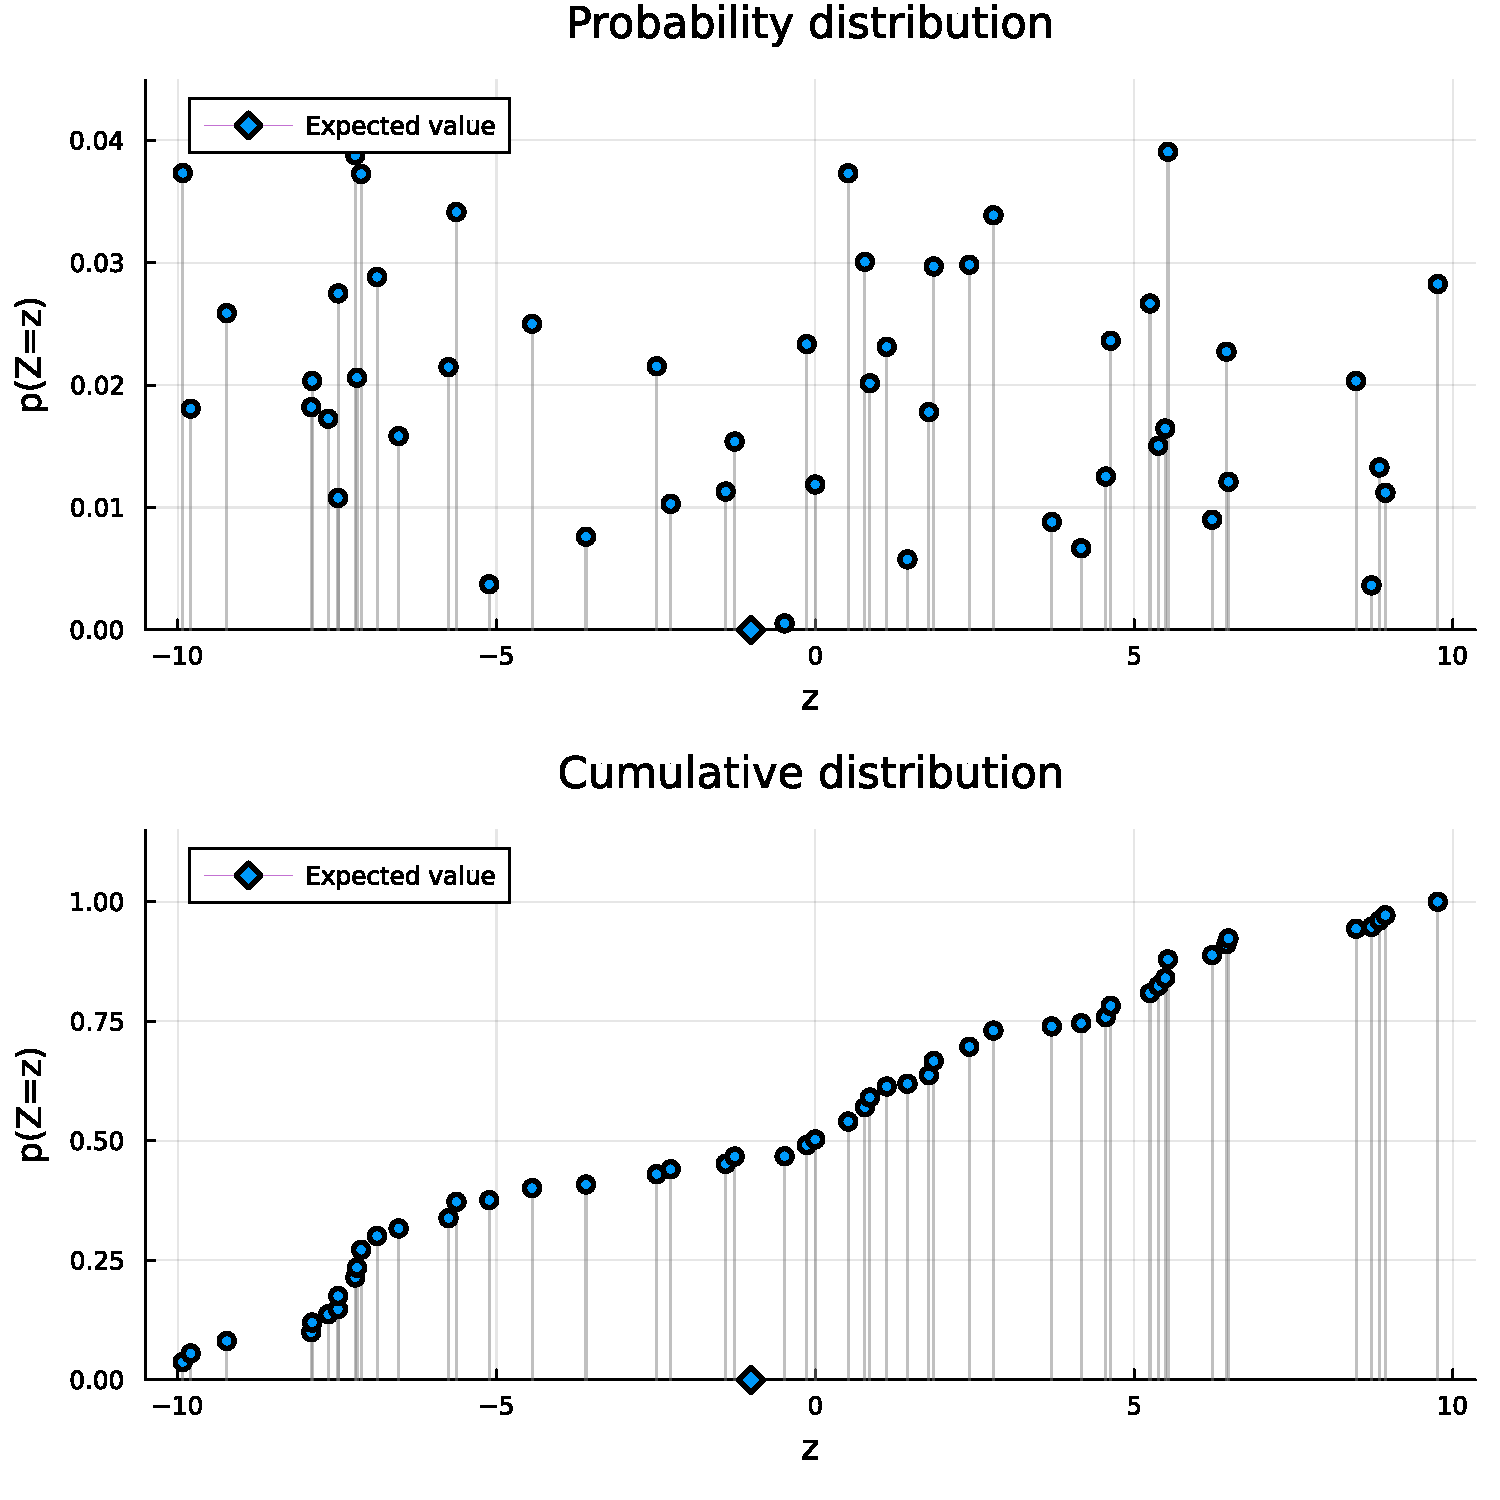
\includegraphics[width=\linewidth]{figures/distributions_1.pdf}
	  \label{fig:sub1}
	\end{subfigure}%
	\begin{subfigure}{.5\textwidth}
	  \centering
	  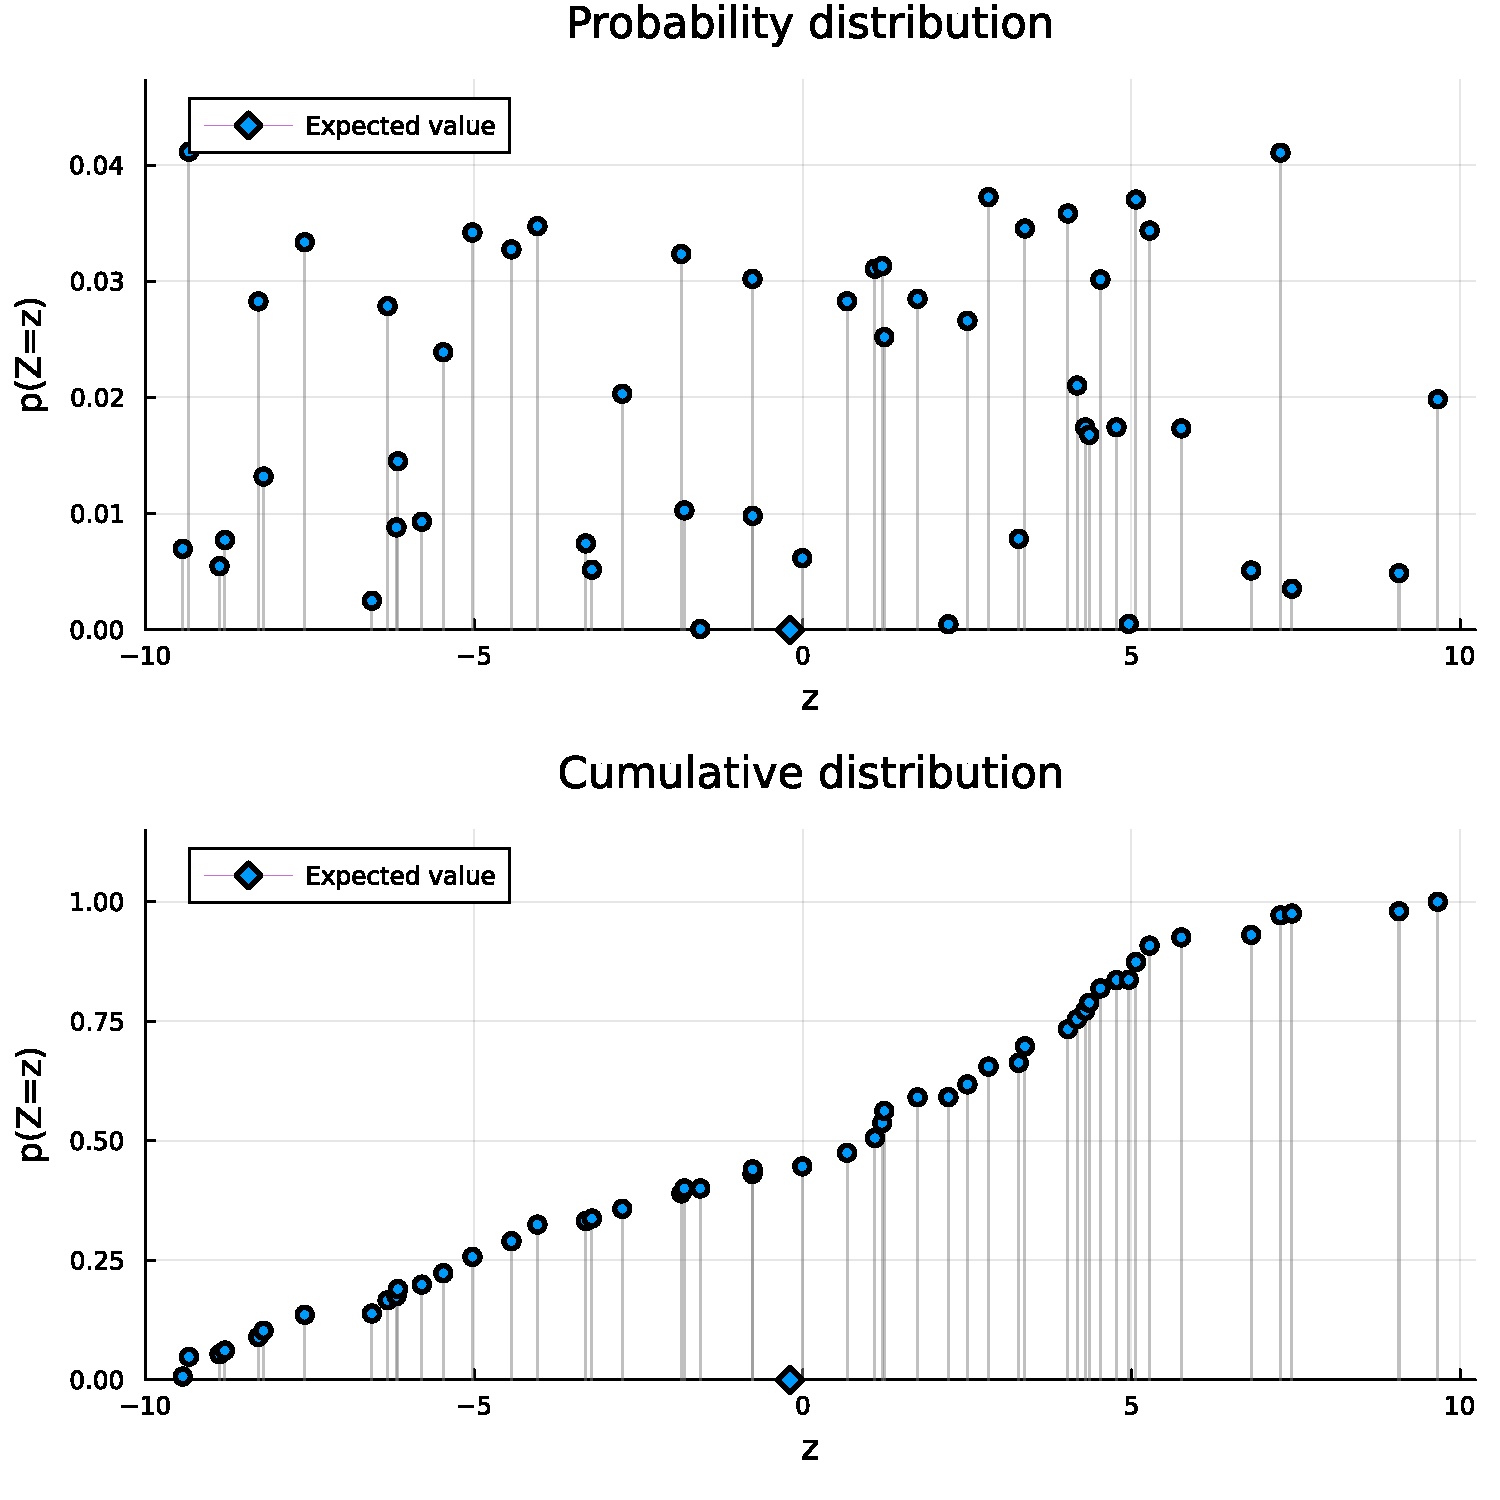
\includegraphics[width=\linewidth]{figures/distributions_10.pdf}
	  \label{fig:sub2}
	\end{subfigure}
	\caption{Comparing two solutions: the solution generating the cost distribution on the left is preferred, as it has a lower expected value}
	\label{fig:test}
	\end{figure}
\end{frame}


\begin{frame}{Measuring risk}

	However, choosing between distributions using their expected values neglects \alert{information about the dispersion}:
	\begin{itemize}
		\item Higher-order statistical moments are disregarded
		\item \alert{Tails} of the cost distribution are often relevant from a decision-making standpoint.	
	\end{itemize}
	
	\pause
	To capture more information about such tails we can define \alert{risk measures} $r : X \to \reals$ such that
		\begin{itemize}
			\item $r$ associates the random variable $F(x, \xi)$ generated by the solution $x$ with a \alert{real-valued risk} $r_\xi(x)$
			\item Analogously, $x'$ can be chosen over $x''$ if $r_\xi\left[F(x', \xi)\right] < r_\xi\left[F(x'', \xi)\right]$
		\end{itemize}
	
\end{frame}


\begin{frame}{Trading off risk and expected return}

	Being \alert{two conflicting objectives}, risk and return are typically considered under a bi-objective standpoint, e.g., using
	\begin{enumerate}[<+->]
		\item \alert{Weighted terms} in the objective function:
		\begin{equation*}	
				\min_x  \mathbb{E}_\xi\left[F(x,\xi)\right] + \beta r_\xi\left[F(x, \xi)\right],
		\end{equation*}
		where $\beta = 0$ represents a risk-neutral stance and risk aversion increases as $\beta \to \infty$;
		\item A \alert{risk exposition budget} $\delta$:
		\begin{align*}	
				\min_x~ & \mathbb{E}_\xi\left[F(x,\xi)\right] \\
				\st & r_\xi\left[F(x, \xi)\right] \le \delta. 
		\end{align*}
	\end{enumerate}
		
\end{frame}


\begin{frame}{Coherent risk measures}

	\alert{\cite{artzner1999coherent}} provides axiomatic definitions for coherent risk measures:
	\begin{enumerate}
		\item {\bf Translation invariance:} $r_\xi\left[F(x, \xi) + a\right] = r_\xi\left[F(x, \xi)\right] + a$ for $a \in \reals$.
		\item {\bf Subadditivity:} $r_\xi\left[F(x', \xi) + F(x'', \xi)\right] \le r_\xi\left[F(x', \xi)\right] + r_\xi\left[F(x'', \xi)\right]$
		\item {\bf Positive homogeneity:	}\hspace{-6pt} $r_\xi\left[F(x, \xi) \times  a\right] = r_\xi\left[F(x, \xi)\right] \times a$ for $a \in \reals$.
		\item {\bf Monotonicity: } if for every $\xi$, we have that $F(x', \xi) \le F(x'', \xi)$, then $r_\xi\left[F(x', \xi)\right] \le r_\xi\left[F(x'', \xi)\right]$
	\end{enumerate}
	
	\pause
	This has been further developed by \alert{\cite{rockafellar2007coherent}}, who establishes the role of \alert{coherence} in optimisation problems. A coherent risk measure:
		\vspace{-6pt}
		\begin{itemize}
			\item Preserves \alert{convexity};
			\item Preserves \alert{certainty};
			\item Is insensitive to \alert{scaling}.	
		\end{itemize}

\end{frame}


\begin{frame}{Conditional value-at-risk}

	The \alert{most widespread risk measure} in the context of optimisation is the Conditional Value-at-Risk (CVaR)
	\vspace{-6pt}
	\begin{itemize}
		\item A \alert{coherent} risk measure widely used in other areas;
		\item Empirical results on its efficacy in production planning: {\small\cite{alem2020practical}}
	\end{itemize}
	
	\pause
	Let $X$ be a random variable and $F_X$ its cumulative distribution function. Then, for a confidence level $\alpha$, the \alert{Value-at-Risk} ($VaR_\alpha$) is defined as
	%
	\begin{equation*}
		VaR_\alpha(X) = \min\{\eta : F_X(\eta)\ge \alpha\}.
	\end{equation*}
	%
	\pause
	The conditional $VaR_\alpha$ represents the \alert{expectation} of $X$ in the \alert{conditional distribution} of its $\alpha$-upper tail, i.e.,
	\begin{equation*}
		CVaR_\alpha(X) = \min_{\eta \in \reals}\braces{\eta + \frac{\mathbb{E}[X - \eta]^+}{(1-\alpha)}},
	\end{equation*}
	where $[\, \cdot \,]^+ = \max\braces{0,\,\cdot\,}$.
	
\end{frame}


\begin{frame}{Conditional value-at-risk}

	\begin{figure}
	\centering
	\begin{subfigure}{.5\textwidth}
	  \centering
	  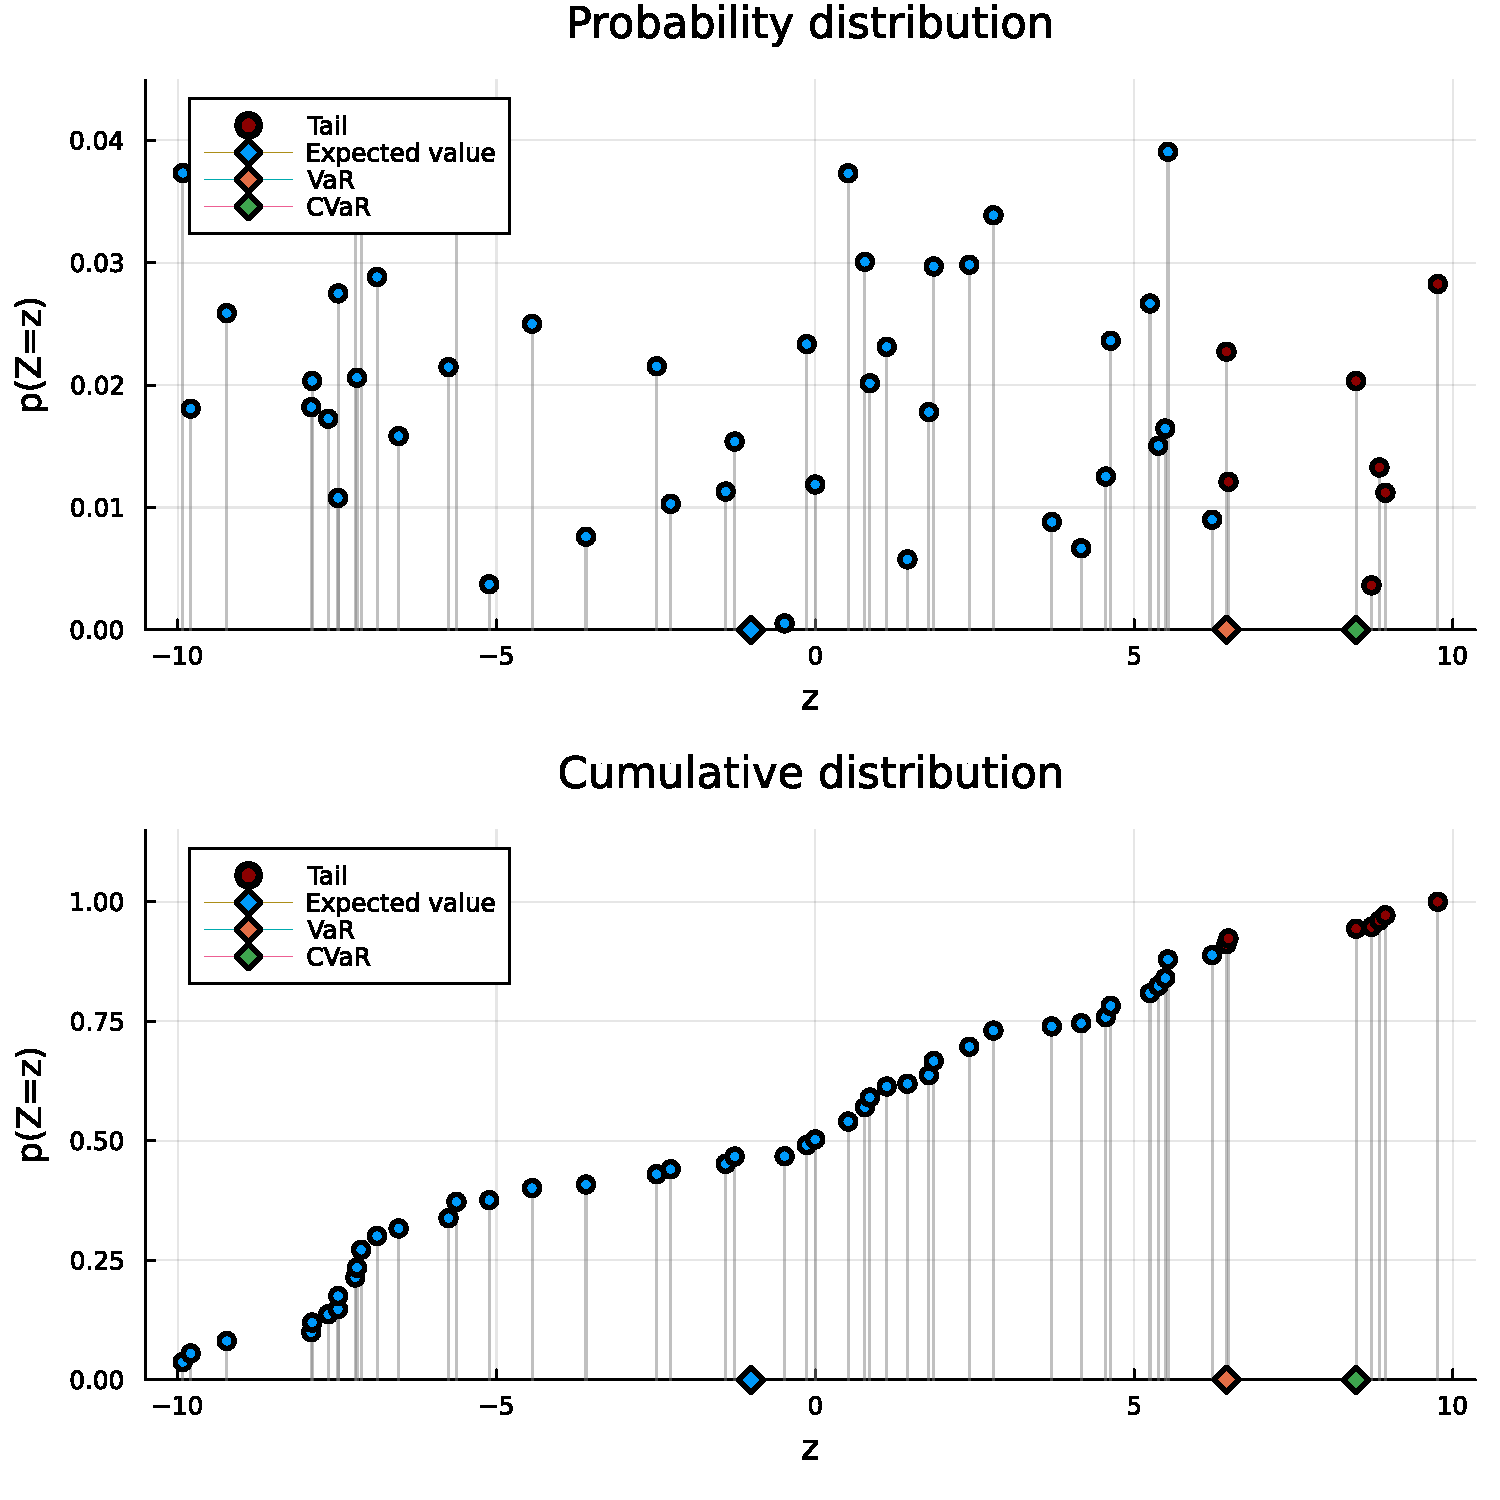
\includegraphics[width=\linewidth]{figures/distributions_CVaR_1.pdf}
	  \label{fig:sub1}
	\end{subfigure}%
	\begin{subfigure}{.5\textwidth}
	  \centering
	  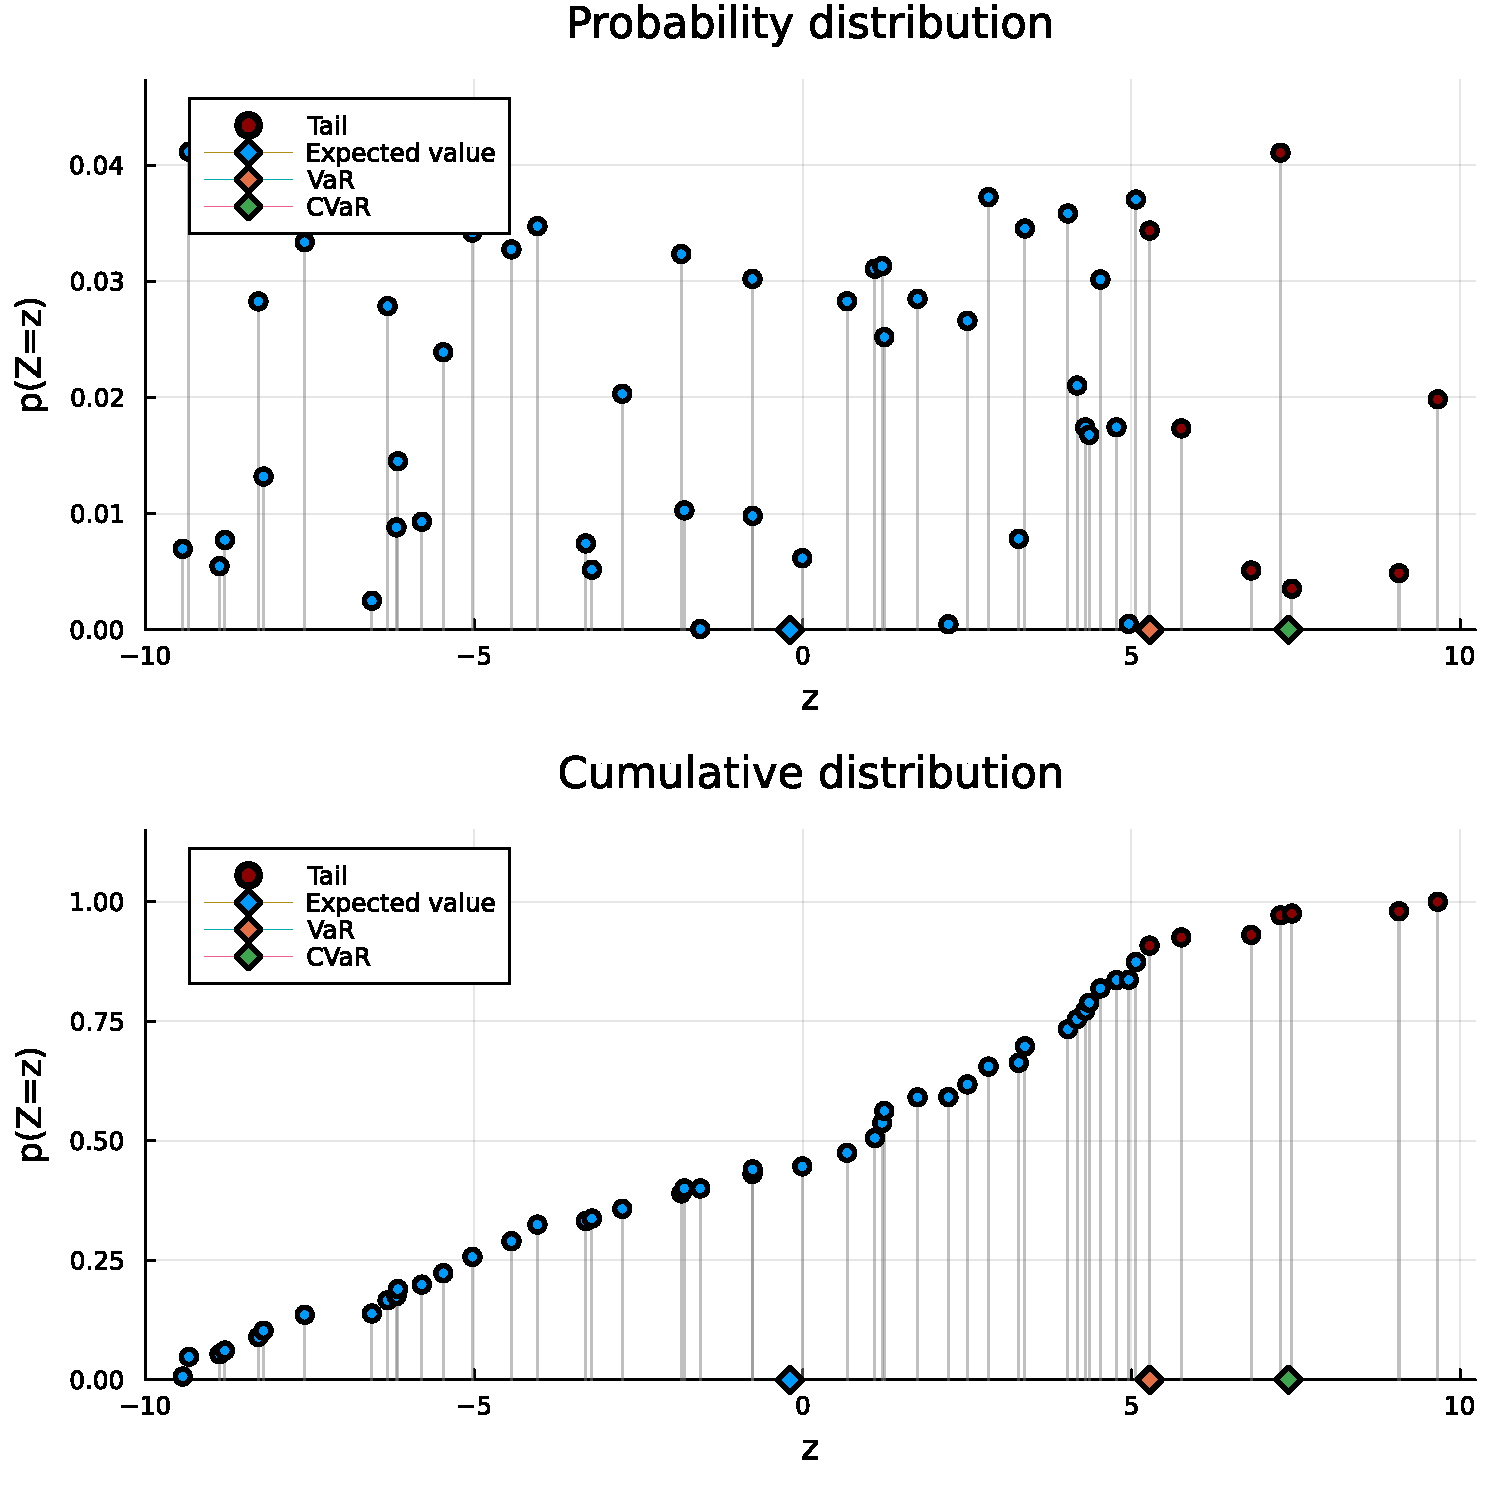
\includegraphics[width=\linewidth]{figures/distributions_CVaR_10.pdf}
	  \label{fig:sub2}
	\end{subfigure}
	\caption{Comparing two solutions: the solution on the right has better (smaller) CVaR$_{90\%}$} 
	\label{fig:test}
	\end{figure}
	
\end{frame}


\begin{frame}{Conditional value-at-risk in SP models}

	One appealing feature of CVaR is its convexity:
	\begin{itemize}
		\item Requires discretisation to handle the expected value;
		\item In the context of optimisation, this means that \alert{no additional binary variables} are needed;
		\item This contrasts with VaR (or chance constraints), which need such variables.
	\end{itemize}
	
	\pause
	Recall our \alert{risk-neutral} scenario-based deterministic equivalent 2SSP:
	%
	\begin{align*}
		\mini  & c^\top x + \sum_{s\in S} P_s q_s^\top y_s \\
		\st	   & Ax = b, x \ge 0 \\
			   & T_sx + W_s y_s = h_s, \ \forall s \in S \\
			   & y_s \ge 0, \ \forall s \in S.
	\end{align*}
	
\end{frame}


\begin{frame}{Conditional value-at-risk in SP models}

	Let us define the following auxiliary terms:
	\vspace{-6pt}
	\begin{itemize}
		\item $\beta \in [0,1]$: weight for the risk term, 
		\item $\alpha$: confidence level;
		\item $\eta \ge 0$: represent the value at risk (VaR); 
		\item $\pi_s \ge 0$, $\forall s \in S$: account for $[X - \eta]^+$. Here $X \equiv c^\top x + q_s^\top y_s$.   
	\end{itemize}
	%
	\pause
	Then, the \alert{risk-averse} scenario-based deterministic equivalent 2SSP is
	\begin{align*}
		\mini  & (1-\beta)\brackets{c^\top x + \sum_{s\in S} P_s q_s^\top y_s} + \beta\brackets{\eta + \frac{\sum_{s \in S} P_s \pi_s}{1-\alpha}} \\
		\st	   & Ax = b, x \ge 0 \\
			   & T_sx + W_s y_s = h_s, \ \forall s \in S \\
			   & \pi_s \ge c^\top x + q_s^\top y_s - \eta, \ \forall s \in S \\
			   & y_s \ge 0, \pi_s \ge 0, \ \forall s \in S \\
			   & \eta \ge 0.
	\end{align*}
\end{frame}


\begin{frame}{Conditional value-at-risk in SP models}

	Some final practical remarks:
	\begin{itemize}[<+->]
		\item Scaling is important. $\beta = 0.5$ is not necessarily a \alert{midpoint} between risk-neutral and risk-averse solutions.
		\item If maximising, pay attention to the \alert{sign} of the additional terms, as they must change accordingly.
		\item CVaR can also be used in \alert{multi-stage} problems (see \cite{SHAPIRO201163})
		\item There are other more recent risk measures for multistage settings (\cite{dowson2022incorporating}) that:
		\begin{itemize}
			\item Behave better (computationally) in \alert{dynamic} settings
			\item Serve as proxy to \alert{other risk-aversion paradigms} (worst-case minimisation or distributional robustness)
		\end{itemize} 
	\end{itemize}

\end{frame}




\begin{frame}[allowframebreaks]{References}

	\bibliographystyle{apalike}
	\bibliography{../aux/references.bib}

\end{frame}